\documentclass[11pt]{article}
\usepackage[utf8]{inputenc}
\usepackage[T1]{fontenc}
\usepackage{fixltx2e}
\usepackage{graphicx}
\usepackage{longtable}
\usepackage{float}
\usepackage{wrapfig}
\usepackage{soul}
\usepackage{textcomp}
\usepackage{marvosym}
\usepackage{wasysym}
\usepackage{latexsym}
\usepackage{amssymb}
\usepackage{hyperref}
\tolerance=1000
\usepackage{fullpage}
\providecommand{\alert}[1]{\textbf{#1}}

\title{Interactive Simulations for CfE Physics}
\author{Craig Roy\vspace{0.5cm}\\Supervisor: Gordon Robb\vspace{0.5cm}\\University of Strathclyde}
\date{}
\begin{document}

\maketitle


\section*{Introduction}
\subsection*{Aim}
The aim of this project was to create interactive simulations to aid the teaching of the new Higher and Advanced Higher Physics Curriculum for Excellence courses.

\subsection*{Motivation}
Since the Curriculum for Excellence programme was implemented, there has been a demand for resources to aid in teaching the new elements of the Higher and Advanced Higher Physics curriculum.

\subsection*{Choice of topics}
The topics chosen for this project were:
\begin{itemize}
\item Special Relativity
\item Particle Accelerators
\item The Doppler Effect
\end{itemize}
These topics were all introduced with the Curriculum for excellence
program. The topics were chosen for this project from a
SUPA\textsuperscript{\cite{supa}} video competition with the same goal of creating more
resources for the new physics courses.

\subsection*{Practical considerations}
The tool used to create the simulations was a program called EjsS or
``Easy Java(Script) Simulations''. EjsS\textsuperscript{\cite{ejs}} is a tool created as a part of the Open Source Physics project. It is designed to make creating computer simulations easy for people such as science teachers and students who are otherwise unfamiliar with programming in Java or JavaScript.

This program was chosen so that simulations could be developed with
relative ease, and so that there is a no barrier to entry for someone
who wants to modify the simulations. Developing the simulations as
Java programs also meets the needs of physics teachers who cannot
access the internet while teaching to view Flash simulations or Java Applets.

\section*{The Simulations}
\subsubsection*{Topic: Our Dynamic Universe}
\subsubsection*{Subtopic: Special relativity}
The first simulation shows a pair of digital clocks. One relatively stationary in a lab, and the other travelling at a relativistic speed specified by the user. The observer is in the reference frame of the lab clock and can observe the slowing down of the moving clock.

\begin{figure}[H]
\centering
\includegraphics[width=.9\linewidth]{./digitalUI.png}
\caption{Screenshot of the digital clock simulation}
\end{figure}

\subsection*{Analogue Clocks}
\subsubsection*{Topic: Our Dynamic Universe}
\subsubsection*{Subtopic: Special relativity}
The second simulation shows a pair of analogue clocks, one of which is
travelling at relativistic speeds. In this simulation, the observer is in the reference frame of the clock travelling at a relativistic speed specified by the user. The user can observe that the stationary clock speeds up as the velocity is increased.

\begin{figure}[H]
\centering
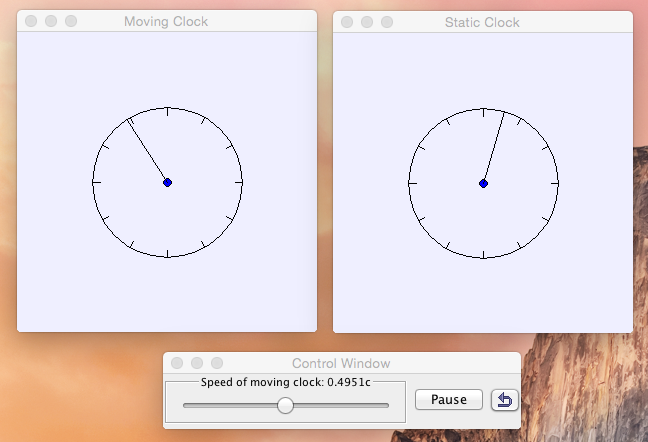
\includegraphics[scale=0.4]{./analogueUI.png}
\caption{Screenshot of the analogue clock simulation}
\end{figure}

\subsection*{Photon Clocks}
\subsubsection*{Topic: Our Dynamic Universe}
\subsubsection*{Subtopic: Special relativity}
 This simulation shows a pair of model photon clocks, with a `photon'
 bouncing between two mirrors. The user is in the reference frame of
 the lab clock. As the user sets the speed of the moving clock, it
 begins to move across the window. At relativistic speeds, the motion
 of the photon appears to slow and the moving photon clock contracts
 in size due to time dilation. This simulation was inspired by a
 similar flash simulation developed by the King's Center for
 Visualisation in Science\textsuperscript{\cite{rocket}}.
\begin{figure}[H]
\centering
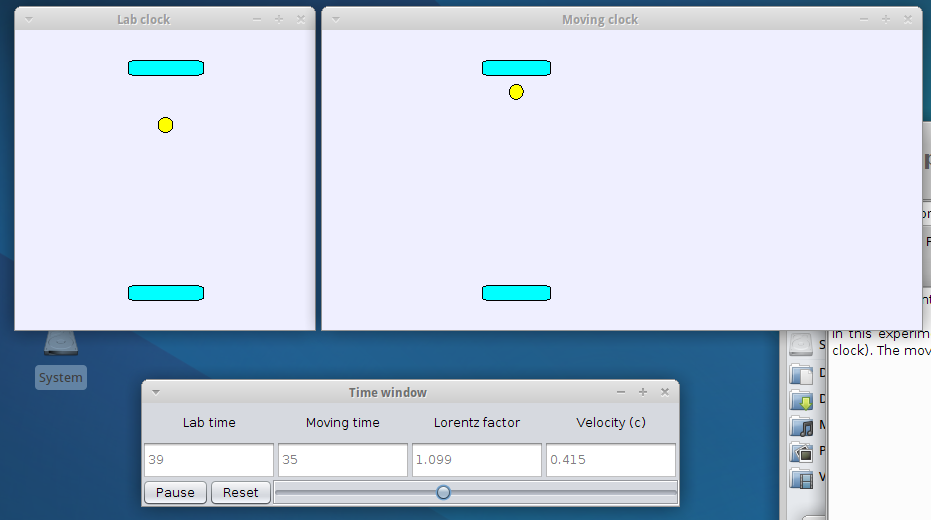
\includegraphics[width=.9\linewidth]{./mirrorUI.png}
\caption{Screenshot of the photon clock simulation}
\end{figure}

\newpage
\subsection*{Cyclotron}
\subsubsection*{Topic: Electromagnetism}
\subsubsection*{Subtopic: Particle Accelerators}
This simulation models a cyclotron particle accelerator which is
relevant to the electromagnetism section of the Advanced Higher
course. The user may set variables such as the strength of the
electric field, the charge of the particle, and the frequency of
oscillation of the electric field and the accelerator will apply the
Lorentz force accordingly. This simulation was inspired by a similar
Java Applet created by the National Taiwan Normal University\textsuperscript{\cite{cyclotron}}.
\begin{figure}[H]
\centering
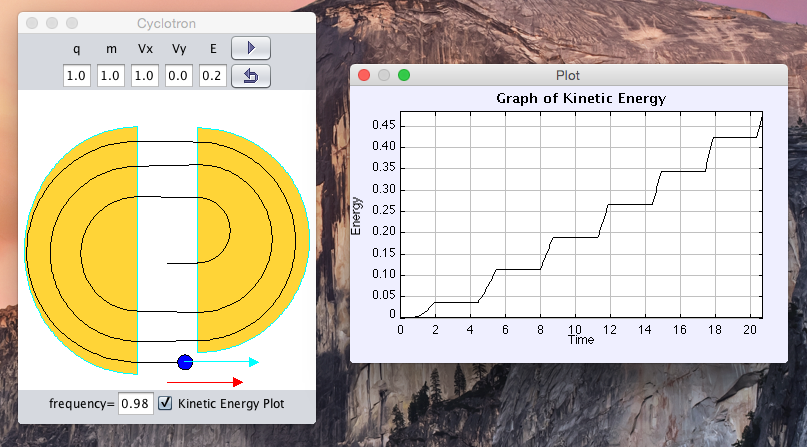
\includegraphics[width=.9\linewidth]{./cycloUI.png}
\caption{Screenshot of the cyclotron simulation}
\end{figure}

\subsection*{Doppler Effect}
\subsubsection*{Topic: Our Dynamic Universe}
\subsubsection*{Subtopic: The Expanding Universe}
This simulation demonstrates the concept of the doppler shift as well
as the concept of using spectroscopy on exoplanets. The simulation
consists of a model exoplanet which is orbiting a star. The planet is
being monitored using spectroscopy. The absorption lines are shown on
a spectrum of visible light at the bottom of the window. The user
chooses the angular velocity of the planet and star, and a Doppler
shift is applied to the spectral lines when the planet is moving
towards the observer or further away. This experiment was inspired by
a similar Flash simulation created by the University of Nebraska-Lincoln\textsuperscript{\cite{doppler}}.
\begin{figure}[H]
\centering
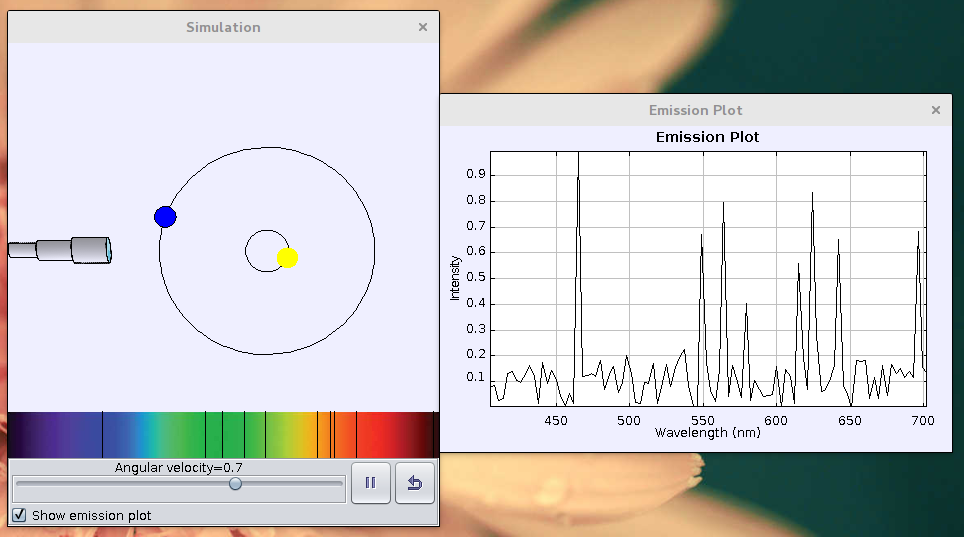
\includegraphics[width=.9\linewidth]{./dopplerUI.png}
\caption{Screenshot of the Doppler Effect simulation}
\end{figure}

\section*{Conclusion}
These simulations were produced during the limited time frame of the
project which was six weeks. Given more time, more of the
syllabus could be covered by such simulations.

All of the simulations produced in this project are open source and
available online\textsuperscript{\cite{repo}}. They can be easily used
or modified by anyone with the inclination.

\section*{Acknowledgements}
We acknowledge and are grateful for partial support from the Scottish Universities Physics Alliance.

\newpage
\begin{thebibliography}{1}

\bibitem{supa}
  SUPA Video Competition,
  \url{http://www.supa.ac.uk/events/supa_videos_2014}

\bibitem{ejs}
  Easy Java(Script) Simulations,
  Francisco Esquembre,
  Open Source Physics,
  \url{http://fem.um.es/Ejs}

\bibitem{rocket}
  Photon Clock,
  Special Relativity,
  King's Center for Visualization in Science,
  \url{http://www.kcvs.ca/site/projects/specialRelativity.html#Photon_Clock}

\bibitem{cyclotron}
  Cyclotron Applet,
  Fu-Kwun Hwang,
  Dept. of physics,
  National Taiwan Normal University,
  Modified: 11/14/2007,
  \url{http://www.schulphysik.de/ntnujava/cyclotron/cyclotron.html}

\bibitem{doppler}
  Extrasolar Planet Radial Velocity Demonstrator,
  University of Nebraska-Lincoln,  \url{http://astro.unl.edu/classaction/animations/light/radialvelocitydemo.html}

\bibitem{repo}
  Github, ComPADRE TBA

\end{thebibliography}

\newpage
\appendix
\section{Special Relativity Report}
\subsection*{Description}
\label{sec-1-1}

This simple time-dilation experiment consists of two `clocks' showing how the time experienced by a clock moving at a relativistic speed specified by the user in the `vField'.
\subsection*{How it works}
\label{sec-1-2}
\subsubsection*{Variables}
\label{sec-1-2-1}

\begin{itemize}
\item \emph{v} is the speed of the moving clock which is specified by the user.
\item \emph{t} is the time shown on the slower, moving clock. It is used to calculate t2.
\item \emph{t2} is the time shown on the static clock, it is calculated for each evolution, by multiplying \emph{t} by the lorentz factor, $\gamma$.
\end{itemize}
\subsubsection*{Evolution}
\label{sec-1-2-2}

The independant variable which is incremented at each evolution is \emph{t}. The animation runs at 20fps, incrementing \emph{t} by 0.05 each time, meaning that \emph{t} increases by 1 second per second.
The variable \emph{t2} increments at $\frac{0.05 \gamma}{frame}$, so $\gamma$ seconds per second.
\subsubsection*{UI}
\label{sec-1-2-3}

In the `control panel' on top, the UI consists of a field in which the user can enter the speed of the moving clock, along with pause and reset buttons.
In the bottom `time panel', the time passed for both the moving and the static clocks is shown. These time fields display the values to one decimal point as a number of seconds.
\section*{Experiment 2: Analogue Clocks}
\label{sec-2}
\subsection*{Description}
\label{sec-2-1}

This experiment is very similar to the previous one, but the information is displayed with model analogue clocks rather than digital displays. Hopefully, this is a clearer demonstration of the concept at hand, and more fun to watch.
In this experiment the moving clock runs at 1 second per second, and the static clock runs faster, whereas in the previous experiment, the static clock ran at 1 second per second and the moving clock ran slower.
\subsection*{How it works}
\label{sec-2-2}
\subsubsection*{Variables}
\label{sec-2-2-1}

\begin{itemize}
\item \emph{v} is the speed of the moving clock which is entered by the user.
\item \emph{tic} is designed to be the independent variable in the ODE page. It is equivalent to the angle in degrees from the 12th hour on the slower moving clock.
\item \emph{a1} is the angle from the 12th hour of the slower moving clock in radians. It is calulated by $\frac{tic \times \pi}{180}$.
\item \emph{x1}, \emph{y1} are the x and y coordinates of the slower clock's hands. They are calculated from \emph{a1} using trigonometry in the fixed relations page.
\item \emph{lorentz} is the lorentz factor, $\gamma$, dependant on the speed entered by the user.
\item \emph{a2} is the angle from the 12th hour of the faster clock in radians. It is found by $\gamma$ \texttimes{} \emph{a1}.
\item \emph{x2}, \emph{y2} are the angles needed for the hands of the faster clock. Calculated using \emph{a2} rather than \emph{a1}.
\end{itemize}
\subsubsection*{Evolution}
\label{sec-2-2-2}

The variables \emph{a1} and \emph{a2} evolve according to the independant variable \emph{tic}. In \emph{a1}, simply converts \emph{tic} to radians and \emph{a2} multiplies \emph{a1} by $\gamma$.
The simulation runs at 6fps, where \emph{tic} is incremented by 1 every frame. This means that the angle of the hand on the slower clock increases by 6\textdegree{} every second. 6\textdegree{} is the angle between 1 second increments on an analogue clock.
From the increments in \emph{a1} and \emph{a2}, the corresponding \emph{x} and \emph{y} values are calculated using the fixed relations $x = -0.5\cos(a)$ and $y = 0.5\sin(a)$.
\subsubsection*{UI}
\label{sec-2-2-3}

The experiments UI consists of three windows:
\begin{itemize}
\item \emph{Spaceship Clock} shows time moving at 1 second per second in the moving rest frame.
\item \emph{Earth Clock} shows time in the static observer frame accelerated by a lorentz factor.
\item \emph{Control Panel} contains a field for the user to input the speed of the moving (spaceship) frame, a play/pause button and a reset button.
\end{itemize}
\section*{Experiment 3: Photon Clock}
\label{sec-3}
\subsection*{Description}
\label{sec-3-1}

This experiment involves the concept of a photon clock. A photon clock is a device which measures the passage of time when a photon hits a sensor.

In this experiment there is a stationary clock (the lab clock) and a moving photon clock (the moving clock) 
   
\subsection*{How to use it}
\label{sec-3-2}

The slider can be used to adjust the speed of the clock in the moving frame. Observe how at speeds very close to the speed of light, the width of the moving photon clock changes.
The times measured by the two clocks are shown in a third window, and so is the Lorentz factor of the second clock and the speed.
\subsection*{How it works}
\label{sec-3-3}
\subsubsection*{Variables}
\label{sec-3-3-1}
\begin{itemize}

\item Simulation variables
\label{sec-3-3-1-1}%
\begin{itemize}
\item \emph{x, vx} are the position and velocity of the moving photon clock system along the x-axis within the frame. The \emph{x} position of the clock is incremented by $vx\dot dt$.
\item \emph{y, vy} are the position and velocity of the photon in the y-axis for the lab clock. \emph{y} is incremented by $vy\dot dt$ for each evolution of the system.
\item \emph{y2, vy2} are the position and velocity of the photon in the y-axis for the moving photon clock system. \emph{y2} is incremented by $vy2\dot dt2$ each evolution of the system.
\item \emph{lorentz} is the value of the Lorentz factor for the moving clock based on the speed of the clock as specified by the user
\item \emph{t} is the time observed by the lab clock.
\item \emph{dt} is the interval in which the lab clock is incremented.
\item \emph{t2} is the time observed by the moving clock.
\item \emph{dt2} is the interval with which the variables in the moving clock system are incremented. It is defined as $\frac{dt}{\gamma}$.
\end{itemize}


\item Length scaling variables
\label{sec-3-3-1-2}%
\begin{itemize}
\item \emph{mirror} is the width of the mirrors in the moving clock window. It is a fixed relation $\frac{2.5}{\gamma}$ so it varies with the speed of the system in order to demonstrate length contraction.
\item \emph{photon} is the width of the photon in the moving clock window. It is of the fixed relation $\frac{0.5}{\gamma}$ so that it also shrinks at high speeds in order to demonstrate length contraction.
\item \emph{upper} is point at which the photon should hit the upper mirror and start moving in the opposite direction.
\item \emph{lower} is the point at which the photon should hit the lower mirror and start moving in the opposite direction.
\end{itemize}
\end{itemize} % ends low level
\subsubsection*{Evolution}
\label{sec-3-3-2}

    Like the previous simulations, this simulation runs at 20fps. The evolution of this system is specified with code, rather than ODEs. There are two time variables \emph{t} and \emph{t2}. As the system evolves, \emph{t} is incremented in real time and \emph{t2} is incremented by $t2 = \frac{real time}{\gamma}$.

    The x-coordinate for the moving clock system simply increases by $vx\dot dt$ on each evolution, the y-coordinate for the moving system similarly increases by $vy\dot dt$.
\subsubsection*{UI}
\label{sec-3-3-3}

The UI consists of three frames:
\begin{itemize}

\item Lab clock frame\\
\label{sec-3-3-3-1}%
The lab clock frame consists of two mirrors with a photon bouncing between them.

\item Moving clock frame\\
\label{sec-3-3-3-2}%
The moving clock frame consists of a photon clock just like in the lab clock frame, but the frame is twice as wide, and as such, the scaling factors in the x axis for the objects are half the value as in the lab clock frame.

This whole system begins to move when the simulation is started and the speed is greater than 0c.

\item Time frame\\
\label{sec-3-3-3-3}%
The timing frame consists of a series of fields showing values of variables and a velocity slider.

\begin{itemize}
\item \emph{Velocity slider} is the widget used to increase the velocity of the moving clock system. It has a maximum value of 1c and a minumum value of 0c. It's value is shown by the velocity field.
\item \emph{Lab time field} shows the time observed on the photon clock which is at rest in the lab.
\item \emph{Moving time field} shows the time observed on a photon clock which is moving away from the lab at a relativistic speed specified by the slider.
\item \emph{Lorentz factor field} shows the Lorentz factor used in making the time dilation and length contraction calculations based on the speed of the moving clock.
\item \emph{Velocity field} shows the velocity of the moving clock as a fraction of c.
\end{itemize}
\end{itemize} % ends low level


\newpage
\section{Cyclotron Report}
\subsection*{Description}
\label{sec-1-1}

This experiment simulates a kind of particle accelerator called a
cyclotron. A cyclotron operates by applying an alternating electric
field between two D-shaped metal structures referred to as
``Dees''. This causes a static particle between the Dees to enter one of
the Dees where it is then shielded from the electric field, but
exposed to a magnetic field within the Dee. This magnetic field
causes the particle's trajectory to rotate so that it then leaves the Dee and reenters the electric field, increasing its velocity and thus putting it in a wider and wider spiral until the particle exits the cyclotron entirely.

This experiment allows the user to observe the effects of adjusting
the frequency at which the electric field oscillates in the
cyclotron. It also allows the user to change the initial velocity of
the particle, the charge and the mass.
\subsection*{How to use it}
\label{sec-1-2}

Along the top of the simulation window, the editable fields for the
values of charge, x and y components of the velocity are shown, along
with the play/pause and reset buttons.
The cyclotron frequency is the field displayed at the bottom of the
window. A plot of the kinetic energy can be shown by clicking the
``Kinetic Energy Plot'' checkbox at the bottom of the screen.
\subsection*{How it works}
\label{sec-1-3}
\subsubsection*{Variables}
\label{sec-1-3-1}
\begin{itemize}

\item Var table
\label{sec-1-3-1-1}%
\begin{itemize}
\item \emph{b} is the magnetic field vector.
\item \emph{x, y} are the x and y positions of the particle.
\item \emph{vx, vy} are the velocity of the particle in the x and y directions respectively.
\item \emph{q} is the charge of the particle in the simulation. It is initially
  set to 1, so that the particle acts as a proton.
\item \emph{m} is the mass of the particle in the simulation.
\item \emph{t} is the time variable of the system.
\end{itemize}

\item Plotting
\label{sec-1-3-1-2}%
\begin{itemize}
\item \emph{ke} is the kinetic energy of the system, given by $ke = \frac{1}{2}mv^2$.
\item \emph{fx} is the force acting on the particle in the x direction due to
  the magnetic field.
\item \emph{fy} is the force acting on the particle in the y direction due to
  the magnetic field.
\item \emph{showPlot} is the variable behind the ``Kinetic Energy Plot'' checkbox.
\end{itemize}


\item E field
\label{sec-1-3-1-3}%
\begin{itemize}
\item \emph{e} is the electric field vector.
\item \emph{freq} is the frequency at which the electric field direction oscillates.
\item \emph{amp} is the magnitude of the electromagnetic field.
\end{itemize}


\item Semicircle
\label{sec-1-3-1-4}%
\begin{itemize}
\item \emph{semiCircX} is the array of points used to plot one of the Dees
  along the x-axis.
\item \emph{semiCircY} is the array of points used to plot one of the Dees
  along the y-axis.
\item \emph{r} is the radius of the semicircle.
\end{itemize}

\end{itemize} % ends low level
\subsubsection*{Initialisation}
\label{sec-1-3-2}

The initialisation section of the simulation is used to populate the
arrays of points which are used to plot the semicircle using the
custom method \emph{getX}.
\subsubsection*{Evolution}
\label{sec-1-3-3}

The evolution page sets up a couple of ODEs such that the rate and which \emph{x} and \emph{y} increase are equal to \emph{vx} and \emph{vy} respectively.

The rate at which \emph{vx} increases is proportional to the Lorentz force in the
x-direction. If the particle is in one of the Dees then the Lorentz
force is only affected by the magnetic field strength. If the particle
is between the Dees, the Lorentz force is only affected by the
electric field strength. The Lorentz force is calculated using the
custom functions \emph{calcForce} and \emph{eForce}. These values are then
divided by mass of the particle to find the acceleration from the
force.

The rate at which \emph{vy} increases is not affected by the electric field
strength, so it is calculated using \emph{calcForce} when the particle is
in one of the Dees.

The electric field vector \emph{e} is given by the cosine
function, \[ A\cdot\cos{f t} \] where \emph{A} is the variable \emph{amp} and
\emph{f} is the variable \emph{freq}.
\subsubsection*{Custom}
\label{sec-1-3-4}

\begin{itemize}
\item \emph{calcForce} takes arguments of the current x and y position and a
  velocity and returns the Lorentz force acting on the particle due to
  the magnetic field. It uses the function \emph{isInDee} to determine
  whether the particle is in one of the Dees. If the particle is not
  in one of the Dees, the \emph{calcForce} returns zero.
\item \emph{eForce} returns the Lorentz force acting on the particle due to the
  electric field. If the particle is not in the electric field,
  \emph{eForce} returns zero.
\item \emph{getX} is used to plot the Dees. Given a y-coordinate and the radius
  of the circle, it returns the corresponding x-coordinate.
\item \emph{isInDee} is used to determine whether the particle is in a Dee or
  not, by checking the x-coordinate and the y-coordinate.
\end{itemize}
\subsubsection*{Fixed Relations}
\label{sec-1-3-5}

The only fixed relation is to set the kinetic energy, \emph{ke} equal to $\frac{1}{2}mv^2$.
\subsubsection*{UI}
\label{sec-1-3-6}
\begin{itemize}

\item Top panel\\
\label{sec-1-3-6-1}%
The panel along the top consists of various fields and labels, as well
as the play/pause button and the reset button.

\item Drawing panel\\
\label{sec-1-3-6-2}%
This panel consists of the drawn part of the simulation. The
proton/electron particle in the system is represented by a 2dObject
called `particle'.
\begin{itemize}
\item \emph{rightDee} is a shape which is formed using the points in
  \emph{semiCircX} and \emph{semiCircY}. It is shifted to the right by 0.2.
\item \emph{leftDee} is created using the same arrays as for \emph{rightDee}, but it
  is rotated 180\textdegree{}.
\item \emph{eArrow} is the arrow which displays the magnetic field vector. It
  is displayed at the bottom and its size is equal to the variable \emph{e}.
\item \emph{bArrow} is the arrow which shows the Lorentz force due to the
  magnetic field on the particle. It originates from the position of
  the particle and it's size is determined by the variables \emph{fx} and \emph{fy}.
\item \emph{vArrow} is the arrow which shows the velocity of the particle. The
  arrow originates at the particle and its size is determined by the
  variables \emph{vx} and \emph{vy}.
\end{itemize}

\item Bottom panel\\
\label{sec-1-3-6-3}%
The bottom panel contains the label and field for the frequency that
the electric field oscillates, given by the variable \emph{freq}.

\item Plotting dialog\\
\label{sec-1-3-6-4}%
This is the window with the kinetic energy plot on it, with \emph{ke} on
the y-axis and \emph{t} on the x-axis.
\end{itemize} % ends low level


\newpage
\section{Doppler Effect Report}
\section*{Description}
\label{sec-1}

This experiment consists of a spectrometer observing an exoplanet. The
relatively stationary observer will see that the absorption spectra
for the exoplanet differ when it is moving towards and away from them.
\section*{How to use it}
\label{sec-2}

The angular velocity of the planet is set using the slider at the
bottom of the window. The absorption spectra for the exoplanet
are shown above the slider. When the slider is moved so the angular
velocity isn't 0, the absorption spectra will begin to shift.

There is also a plot of the emission spectra for the exoplanet which
can be opened by checking the ``Show emission plot'' checkbox at the
bottom of the window.
\section*{How it works}
\label{sec-3}
\subsection*{Variables}
\label{sec-3-1}

\begin{itemize}
\item \emph{a} is the angle of rotation of the exoplanet from the northern position.
\item \emph{r, r2} are the radius of the path travelled by the exoplanet and
  the radius of the path travelled by the star it orbits respectively.
\item \emph{x, y} are the x and y coordinates of the exoplanet. These
  coordinates are determined from the angle of the planet, \emph{a}, and
  the radius of the path travelled by the exoplanet, \emph{r}.
\item \emph{vx, vy} are the velocity of the exoplanet in the x and y axes
  respectively. They are also calculated from the angle of the planet,
  as well as the angular velocity of the system, \emph{omega}.
\item \emph{t} is the time variable for the evolution of the system.
\item \emph{off} is the offset added to the position of the star-planet
  system to move it to the right of the spectrometer image.
\item \emph{segment} is the two-dimensional array of coordinates for the absorption lines.
\item \emph{posRef} is the array of positions of the absorption lines before
  the Doppler shift is applied.
\item \emph{offset} is the amount which the position of the absorption lines should be offset by the Doppler shift caused by the motion of the planet.
\item \emph{x2, y2} are the x and y positions of the star.
\item \emph{omega} is the angular velocity of both the exoplanet and the star.
\end{itemize}
\subsubsection*{Plotting Variables}
\label{sec-3-1-1}

\begin{itemize}
\item \emph{xPoints, yPoints} are the arrays of coordinates for the points to plot on the emission spectrum plot.
\item \emph{waveOffset} is the amount which the wavelengths of the emission lines should be shifted due to the Doppler effect.
\item \emph{showPlot} is the variable behind the ``Show Emission Plot'' checkbox.
\item \emph{lamRef} is the array of x-coordinates for the points on the graph not considering the Doppler shift.
\end{itemize}
\subsection*{Initialisation}
\label{sec-3-2}

In the initialisation, an array of four random wavelengths between
400nm and 700nm are randomly generated and used to populate the
arrays, \emph{xPoints} and \emph{lamRef}. They are given a corresponding value
in \emph{yPoints} between 0 and 0.2. Then, ten points from the array are
randomly chosen as the absorption spectra and these points are given
corresponding y-coordinates with values between 0.2 and 1. These wavelengths are then scaled down to values
between -1 and 1 for use plotting the absorption lines on the spectrum
of visible light. These are used to populate the two-dimensional
array, \emph{segment}, where the second dimension is the y-coordinate, -1
in order to place the lines at the bottom of the screen.
\subsection*{Evolution}
\label{sec-3-3}
\subsubsection*{Evol Page}
\label{sec-3-3-1}

The first evolution page introduces the relationship between the angle of rotation, \emph{a}, and the angular velocity, \emph{omega}.
\subsubsection*{Spectra}
\label{sec-3-3-2}

For each step of the evolution of the system, this page sets the positions and the points of the spectral lines equal to their reference values plus the appropriate Doppler shift.
\subsection*{Fixed relations}
\label{sec-3-4}

The fixed relations page contains relationships generating x and y coordinates and velocities from the angle of the planet and star.
It also generates the offset for the positions and wavelengths of the absorption spectra based on the magnitude of the velocity in the x-axis.
\subsection*{Custom}
\label{sec-3-5}

\begin{itemize}
\item \emph{positionToWavelength} takes a position on the spectrum between -1 and 1 and converts it to the equivalent wavelength in nanometers (between 400nm and 700nm) for plotting on the graph.
\item \emph{wavelengthToPosition} does the opposite of the \emph{positionToWavelength} method.
\item \emph{randomPosition} generates a random value between -1 and 1 to be used as a position for an absorption line.
\end{itemize}
\subsection*{UI}
\label{sec-3-6}
\subsubsection*{Frames}
\label{sec-3-6-1}

The UI of this experiment consists of two windows: the simulation
window and the plotting window. The plotting window is hidden by
default and is opened with the ``Show emission plot'' checkbox at the
bottom of the simulation window.

The simulation window contains the model exoplanet orbiting a star,
showing their paths. It also shows the absorption lines for the
exoplanet plotted on the spectrum of visible light. It has a slider at
the bottom to change the angular velocity of the planet, as well as
the play/pause button, the reset button and the checkbox to show the
emission spectrum plot.
\subsubsection*{Images}
\label{sec-3-6-2}

This simulation makes use of two images. A drawing of a telescope, to
act as a mock spectrometer, and a picture of the spectrum of visible
light, to be the background for the spectral lines. Both of these
images are freely licensed.


\end{document}
